
\chapter{Information sheet}\label{ch:information_sheet}
The information sheet given to the participants in Study 1 is shown in Figure \ref{fig:informationsheet}. 

\begin{figure}[htp] \centering{
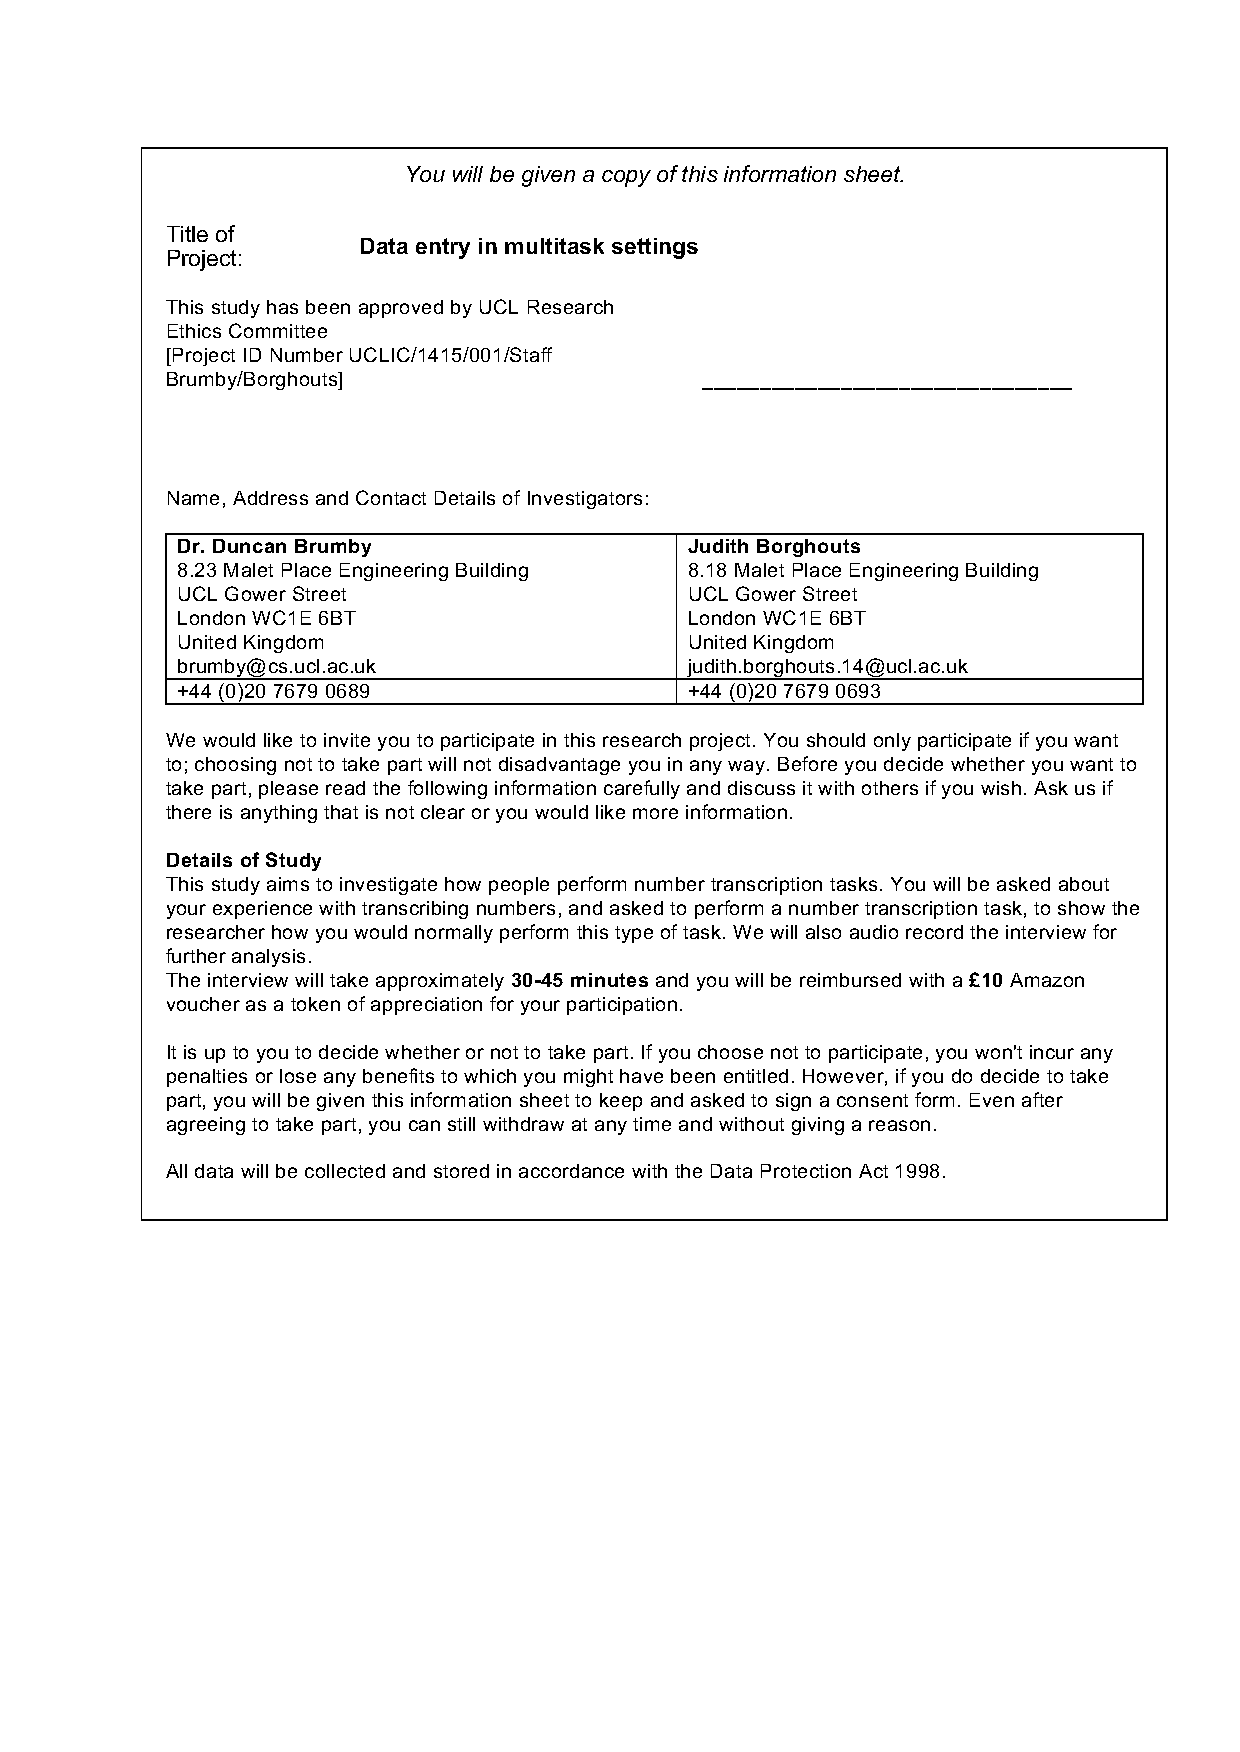
\includegraphics[width=\textwidth,keepaspectratio]{images/Informationsheet.pdf}}
\caption{Information sheet}
\label{fig:informationsheet}
\end{figure} 

\chapter{Consent form}\label{ch:consentform}
The consent form used for Study 1 is shown in Figure \ref{fig:consentform}. 

\begin{figure}[htp] \centering{
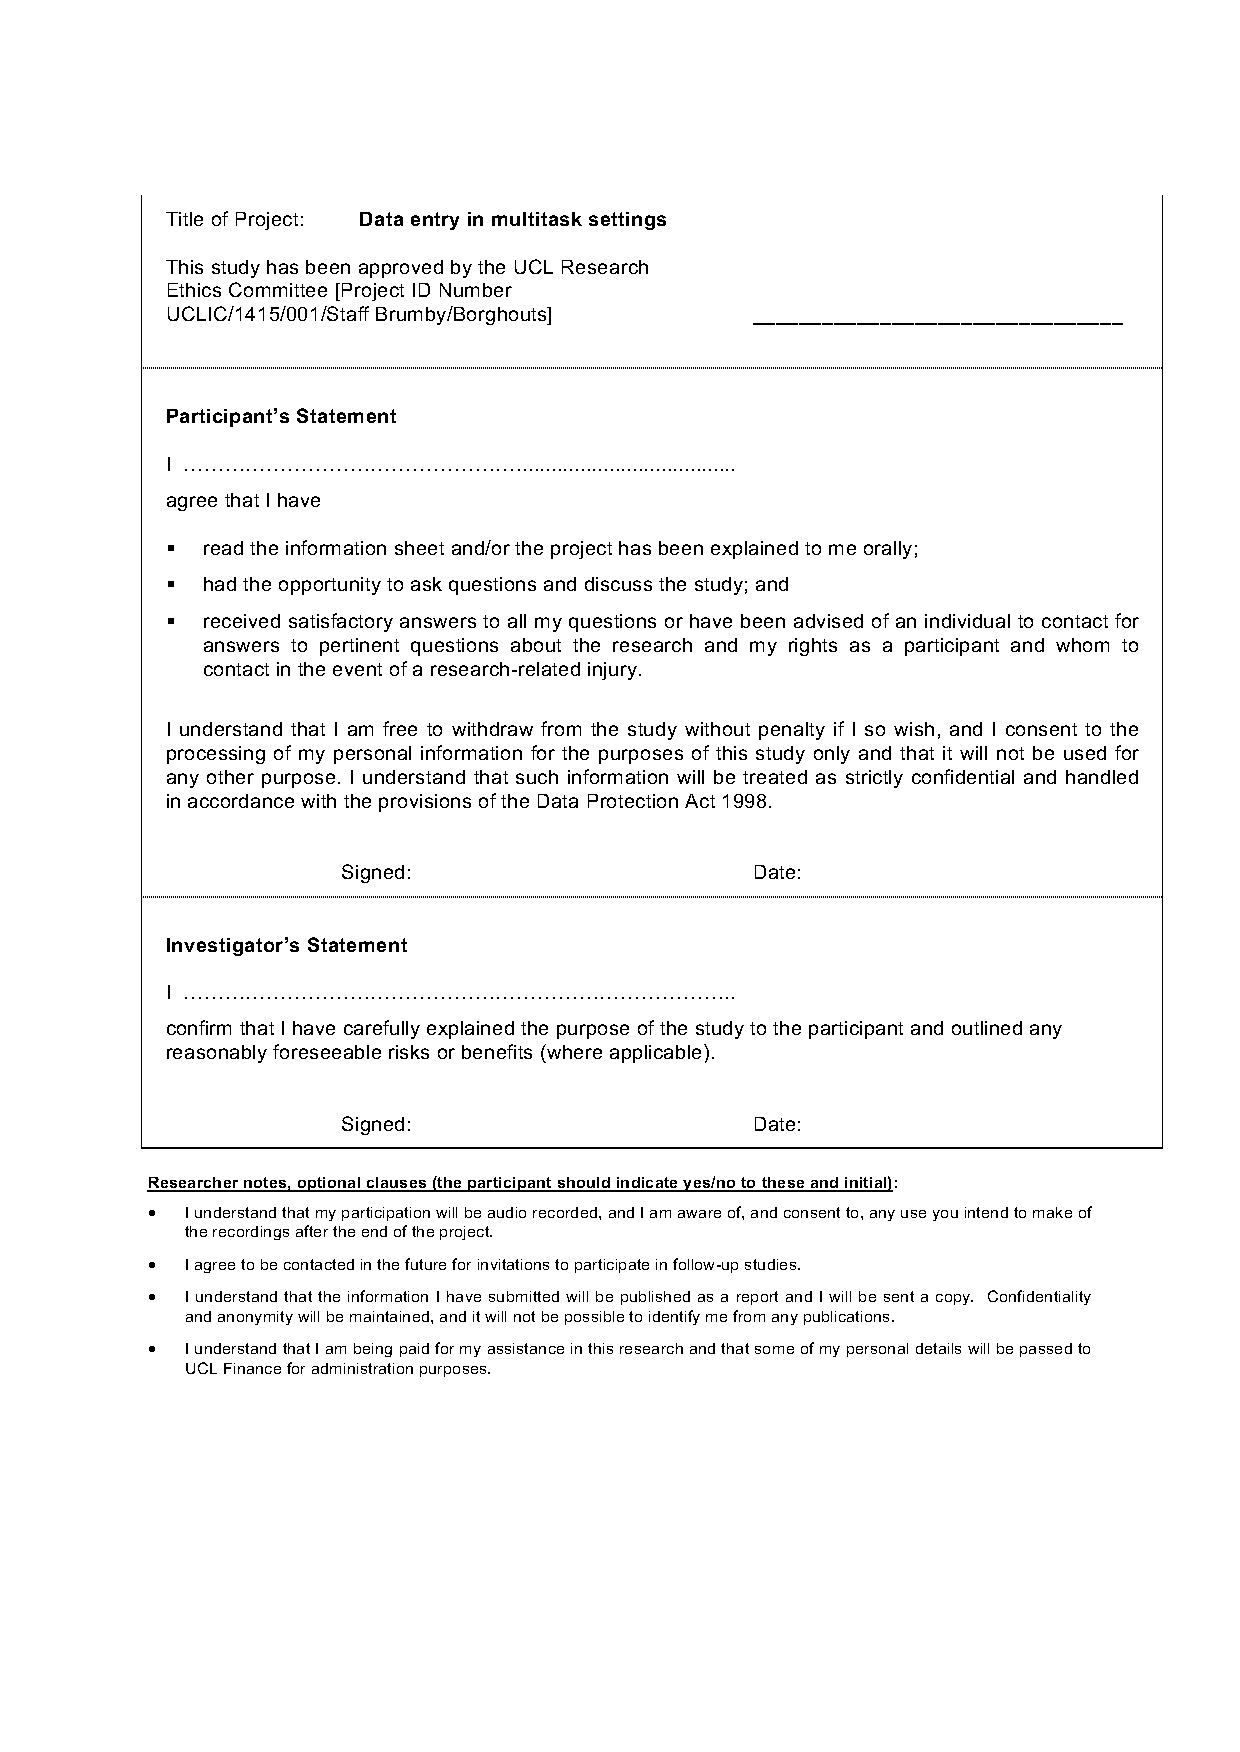
\includegraphics[width=\textwidth,keepaspectratio]{images/Consentform.pdf}}
\caption{Consent form}
\label{fig:consentform}
\end{figure} 

\chapter{Interview script}\label{ch:interviewscript}
The interview script used for Study 1 is given below. This script only served to guide the interview, and does not contain all questions that were asked. Based on what the participant was saying, follow-up questions were asked. 

\subsubsection{Before the interview}
\begin{itemize}
\item 
ensure participant is aware of purpose research 
\item 
explain what will happen
\item 
informed consent
\item 
ask for permission to audio record interview
\end{itemize}
\subsubsection{Work}
\begin{itemize}
\item Tell me something about your work (what do you do)
\item  How many hours per week (full-time/part-time)
\item How long have you been working here (at this company) \item How long have you been doing this type of work
\end{itemize}
\subsubsection{Number entry}
\begin{itemize}
\item  What activities do you do for work that involve transcribing numbers?
e.g. filling in expenses, tax returns, setting up invoices
\item How often do you do this (per day/week)?
\item How many numbers is it roughly that you have to enter?
\item How long do you usually take?
\item What type of numbers? Usually same numbers, or can it be anything?
\item Do you get to enter numbers that are different from your familiar format?
e.g. 2,000 or 2.000; 9/15/14 instead of 15/9/14
\item Do you deal with foreign currencies?
\item Tell me something about how you enter these numbers
\item When do you do these tasks? Immediately when you get them, or save them for later? Morning, afternoon?
\item Does urgency/time pressure influence how you do the task (if so, how)
\item Do you do them in-between other tasks or save a particular part of the day for it?
\item Do you do all tasks all at once, or take rests in between?
(if rests, what do you do? switch to another task, have a coffee, lunch, break, etc.)
\item Do you feel that the way you enter it changes after a while?
e.g. you get better at it so it kind of becomes automatic, or less mentally exhausting? Or is it the opposite, becomes more exhausting?
\item Do you do other things as well during this task
e.g. listening to music, attending to another task
\item Do you sometimes have to briefly store numbers in memory, or calculate them from numbers you already have?
If so, do you use external tools to offload memory?
\item Where do you copy them from? Paper, digital files, combination?
\item Do numbers get checked, to see if they're correct? Do you or anyone else check these numbers?
\item Do you ever get entered numbers from someone else, that you then have to check if they are correct?
\item What is your general experience with transcribing numbers?
e.g. easy, boring, part of the job
\end{itemize}
\subsubsection{Environment}
\begin{itemize}
\item Do you always work in the same environment, or sometimes work in different places, such as at home, or when you're on the train, or working at a cafe? What about number entry tasks?
\item Do you do your work on a desktop, laptop, tablet, anything else? Are some devices harder or easier?
\item How is your desk organized?
\item Do you organise it differently when doing number entry tasks?
\item Do you have notifications on (e.g. e-mail, work-related instant messaging); if you do get new notification, do you attend to it straight away or finish task first?
\item Do you get interrupted in other ways, for example when the phone is ringing, or when a colleague or your boss asks you something? How do you deal with these interruptions? What is your experience with these interruptions?
\item Critical incident: Has there ever been an incident where a mistake in entering a number went undetected, and was discovered later on?
\end{itemize}
\subsubsection{Demonstration}
\begin{itemize}
\item Could you show me the software you use to transcribe numbers?
What is your experience with this system, works well?
(If negative, how do you deal with that? do you use any strategies to make it more optimal for yourself?)
\item Do you feel confident entering the numbers?
\item How do you place your windows?
\item Could you show me how you perform a typical number transcription task (do it how you would normally); if you feel uncomfortable about sharing work data, you can enter any type of numbers, as long as it somewhat resembles data you would normally enter for work
\end{itemize}
\subsubsection{After the interview}
\begin{itemize}
\item Thank participant
\item explain what will happen to their data
\item do they have any more questions
\item clarify when they will be compensated
\item Ask if participant knows any further people who might be suitable and willing to participate
\end{itemize}
